%%%%%%%%%%%%%%%%%%%%%%%%%%%%%%%%%%%%%%%%%
% Short Sectioned Assignment LaTeX Template Version 1.0 (5/5/12)
% This template has been downloaded from: http://www.LaTeXTemplates.com
% Original author:  Frits Wenneker (http://www.howtotex.com)
% License: CC BY-NC-SA 3.0 (http://creativecommons.org/licenses/by-nc-sa/3.0/)
%%%%%%%%%%%%%%%%%%%%%%%%%%%%%%%%%%%%%%%%%

%----------------------------------------------------------------------------------------
%	PACKAGES AND OTHER DOCUMENT CONFIGURATIONS
%----------------------------------------------------------------------------------------

\documentclass[paper=a4, fontsize=11pt]{scrartcl} % A4 paper and 11pt font size

% ---- Entrada y salida de texto -----

\usepackage[T1]{fontenc} % Use 8-bit encoding that has 256 glyphs
\usepackage[utf8]{inputenc}
%\usepackage{fourier} % Use the Adobe Utopia font for the document - comment this line to return to the LaTeX default

% ---- Idioma --------

\usepackage[spanish, es-tabla]{babel} % Selecciona el español para palabras introducidas automáticamente, p.ej. "septiembre" en la fecha y especifica que se use la palabra Tabla en vez de Cuadro

% ---- Otros paquetes ----

\usepackage{url} % ,href} %para incluir URLs e hipervínculos dentro del texto (aunque hay que instalar href)
\usepackage{amsmath,amsfonts,amsthm} % Math packages
%\usepackage{graphics,graphicx, floatrow} %para incluir imágenes y notas en las imágenes
\usepackage{graphics,graphicx, float} %para incluir imágenes y colocarlas

\usepackage{listings}	%para incluir remarcado para comandos bash

% Para hacer tablas comlejas
%\usepackage{multirow}
%\usepackage{threeparttable}

%\usepackage{sectsty} % Allows customizing section commands
%\allsectionsfont{\centering \normalfont\scshape} % Make all sections centered, the default font and small caps

\usepackage{fancyhdr} % Custom headers and footers
\pagestyle{fancyplain} % Makes all pages in the document conform to the custom headers and footers
\fancyhead{} % No page header - if you want one, create it in the same way as the footers below
\fancyfoot[L]{} % Empty left footer
\fancyfoot[C]{} % Empty center footer
\fancyfoot[R]{\thepage} % Page numbering for right footer
\renewcommand{\headrulewidth}{0pt} % Remove header underlines
\renewcommand{\footrulewidth}{0pt} % Remove footer underlines
\setlength{\headheight}{13.6pt} % Customize the height of the header

\numberwithin{equation}{section} % Number equations within sections (i.e. 1.1, 1.2, 2.1, 2.2 instead of 1, 2, 3, 4)
\numberwithin{figure}{section} % Number figures within sections (i.e. 1.1, 1.2, 2.1, 2.2 instead of 1, 2, 3, 4)
\numberwithin{table}{section} % Number tables within sections (i.e. 1.1, 1.2, 2.1, 2.2 instead of 1, 2, 3, 4)

\setlength\parindent{0pt} % Removes all indentation from paragraphs - comment this line for an assignment with lots of text

\newcommand{\horrule}[1]{\rule{\linewidth}{#1}} % Create horizontal rule command with 1 argument of height

\usepackage{booktabs}
\usepackage{tabularx}
\usepackage{multicol} 
\usepackage{hyperref}

%----------------------------------------------------------------------------------------
%	TÍTULO Y DATOS DEL ALUMNO
%----------------------------------------------------------------------------------------

\title{
	\normalfont \normalsize 
	\textsc{\textbf{Gestión de la información en la Web (2020-2021)} \\ Máster en
		ingeniería informática \\ Universidad de Granada} \\ [25pt] % Your university,
	%school and/or department name(s)
	\horrule{0.5pt} \\[0.4cm] % Thin top horizontal rule
	\huge Práctica 4: Caso Práctico de Análisis y Evaluación de Redes en Twitter en
	Filtrado Colaborativo \\ % The assignment title
	\horrule{2pt} \\[0.5cm] % Thick bottom horizontal rule
}
\author{Manuel Orantes Taboada \\ \\ manuelorantes96@gmail.com \\
	morantes96@correo.ugr.es \\ 77150692K} % Nombre y apellidos

\date{\normalsize\today} % Incluye la fecha actual

%----------------------------------------------------------------------------------------
% DOCUMENTO
%----------------------------------------------------------------------------------------

\begin{document}
	
	\maketitle % Muestra el Título
	
	\newpage %inserta un salto de página
	
	\tableofcontents % para generar el índice de contenidos
	
	\newpage
	
\section{Selección del medio social, definición de la pregunta y obtención del conjunto datos asociado}

En primer lugar, indicar que se ha utilizado Twitter como red social de la cual
obtener información. A parte de esto, para ponernos en situación, mis preguntas
irán referidas al partido de la final de la Champions que tuvo lugar en la
pasada noche del sábado 29 de Mayo. Esta se disputó en Oporto entre el
Manchester City y el Chelsea. Los tweets además fueron recogido en torno a las
21:45, cuando se iba a dar el descanso del partido. En ese momento, el Chelsea
acababa de marcar un gol y por consiguiente, adelantarse en el encuentro. 
\\\\
Dicho esto, las preguntas que quiero responder con este estudio son las
siguientes, siendo la primera la que considero más probable que se consiga y la
última la menos probable (a priori):
\begin{itemize}
	\item ¿Los usuarios @ChelseaFC (cuenta oficial del Chelsea) y @ManCity (cuenta
	oficial del Manchester City) son los más relevantes sobre el tema \#UCLfinal
	(hastag del partido en cuestión) del día 29 de Mayo a las 21:45?
	\item ¿Podría localizar a la cuenta @kaihavertz29 (cuenta oficial del jugador
	que acababa de marcar el gol)?
	\item ¿Se podrán diferenciar la comunidad del Chelsea de la del Manchester
	City?
\end{itemize}

El conjunto de datos se obtuvo a raíz del plugin de Gephi, creando previamente
las credenciales necesarias para poder obtener datos de Twitter. Los nodos representan cuentas de Twitter mientras que las aristas son retwittes, me gusta y comentarios entre estas cuentas.

\section{Construcción de la red social a analizar y visualizar}

La recolección de datos fue muy rápida, dato que pienso que será relevante al
final del estudio. Como era un tema candente, en menos de un minuto obtuve de la
API de twitter 12330 nodos y 25160 aristas. Por este motivo, realice un
tratamiento previo de los datos, para reducir este número de nodos y aristas y
así quitar del visualizado mucha información que, muy probablemente, no será
100\% relevante.
\\\\
Para ello, apliqué dos filtros previos, el filtro de la componente gigante y
otro que filtraba por el grado del nodo, obteniendo los nodos que tuvieran al
menos grado 5. 

\begin{figure}[H]
	\centering
	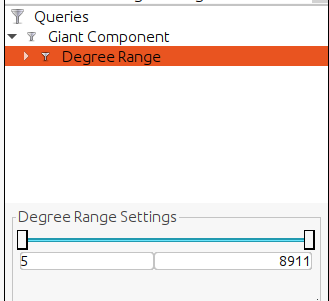
\includegraphics[width=0.2\linewidth]{Imagenes/screenshot001}
\end{figure}


El resultado fue obtener 598 nodos y 2497 aristas, reflejando esto un 4,85\% de
los nodos totales y menos de un 10\% de las aristas totales.

\begin{figure}[H]
	\centering
	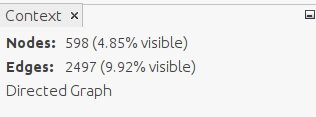
\includegraphics[width=0.35\linewidth]{Imagenes/screenshot002}
\end{figure}

Una vez obtenidos los datos, los exporté a un archivo csv para que fuera más
fácil trabajar con ellos. Además, como los nodos no tenían etiquetas, copié su
id (nombre de usuario) a las etiquetas, de modo que ya podemos diferenciar los
nodos y ponerles un nombre.


\section{Cálculo de los valores de las medidas de análisis}

\begin{center}
	\begin{tabular}{ c c }
		Número de nodos: & 598  \\ 
		Número de enlaces: & 2497  \\  
		Densidad: & 0.007  \\
		Grado medio: & 4.176 \\  
		Diámetro: & 6 \\
		Distancia media: &  1.67 \\ 
		Distancia media para la red aleatoria equivalente: & 4.47 \\ 
		Coeficiente de clustering medio: & 0.113 \\ 
		Coeficiente de clustering medio para la red aleatoria equivalente: & 0.007 \\ 
		Conectividad: & 100\%
	\end{tabular}
\end{center}

\subsection{Grado medio}
Cabe destacar, que aunque hemos eliminado de la red grande los nodos de grado menor que cinco. Estos eran una inmensa mayoría. Pero, a partir de 5, ya no eran tanto los nodos que tenían poco grado, y es por eso que obtenemos un grado relativamente alto.


\subsection{Diámetro y distancia media}
Como podemos ver en la imagen de abajo, la red tiene un diámetro muy muy bajo, y la distancia media de hecho es menor de dos. Esto se debe a que debido a que el tema candente siempre giraba entorno a dos o tres actores principales, y el hecho de recolectar los datos en un espacio temporal muy pequeño, haga que todo apunte fácilmente a unos nodos centrales, que seguiremos viendo a lo largo de la práctica.

\newpage
\subsection{Conectividad de la red}

En este caso, por la manera en la que he realizado la reducción de los datos, no tiene sentido calcular la conectividad de la red, ya que toda la red es una única componente conexa, y el porcentaje de la componente gigante es 100\%. Para este caso, voy a calcular la conectividad de la primera red, antes de realizarle las transformaciones.
\\\\
En este caso, hay 849 componentes conexas. En cuanto a los números de la componente gigante, este ostenta el 79,6\% de los nodos y el 87,43\% de las aristas.

\section{Determinación de las propiedades de la red}
\subsection{Distribución de grado}
\subsubsection{Entrada}
\begin{figure}[H]
	\centering
	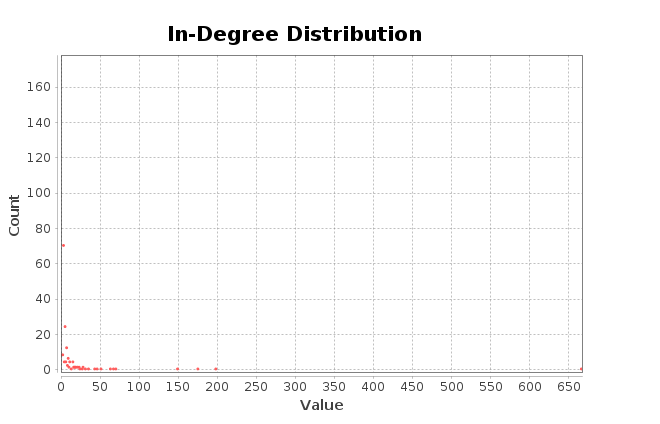
\includegraphics[width=0.6\linewidth]{Imagenes/screenshot005}
\end{figure}

\subsubsection{Salida}
\begin{figure}[H]
	\centering
	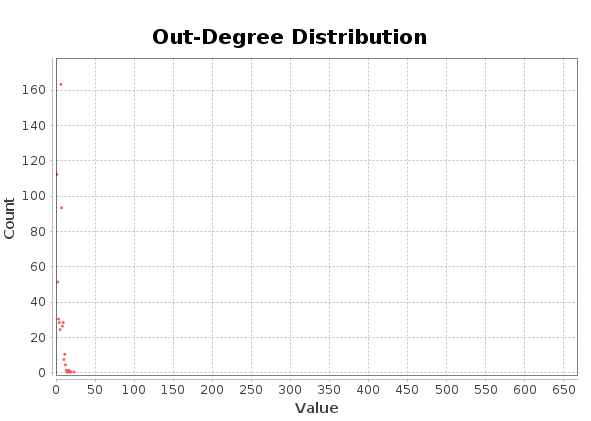
\includegraphics[width=0.6\linewidth]{Imagenes/screenshot006}
\end{figure}

\subsection{¿La red es libre de escala?}

Veamos las dos distribuciones anteriores. Obviamente se puede imaginar que la distribución sigue más o menos una función de una potencia, pero, es claro, al menos en el caso de la red de salidas, que no es una red libre de escala. En el caso de la red de entrada, podría ser más dudoso, llegándose a observar la ley de la potencia en cierto modo.

\subsection{Distribución de distancia}
\begin{figure}[H]
	\centering
	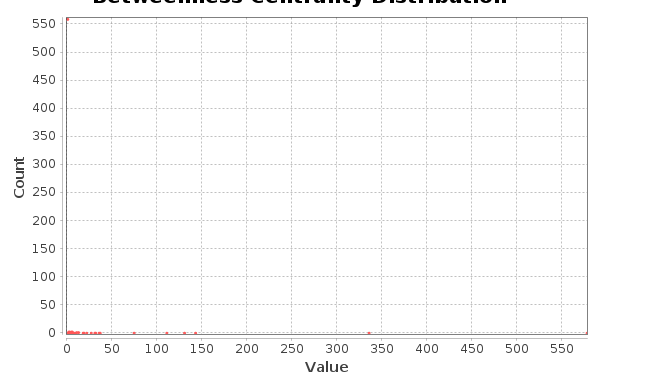
\includegraphics[width=0.6\linewidth]{Imagenes/screenshot008}
\end{figure}

Diría, viendo la gráfica objetivo, que es un mundo ultra-pequeño, ya que la escala parece menor que la logarítmica.

\subsection{Distribución de coeficientes de clustering}

En la siguiente imagen, muestro la distribución de los coeficientes de clustering. La verdad es que no sé interpretar esa imagen, pero se ve que el clustering medio es muy cercano a cero, lo que puede influir en la propia distribución.

\begin{figure}[H]
	\centering
	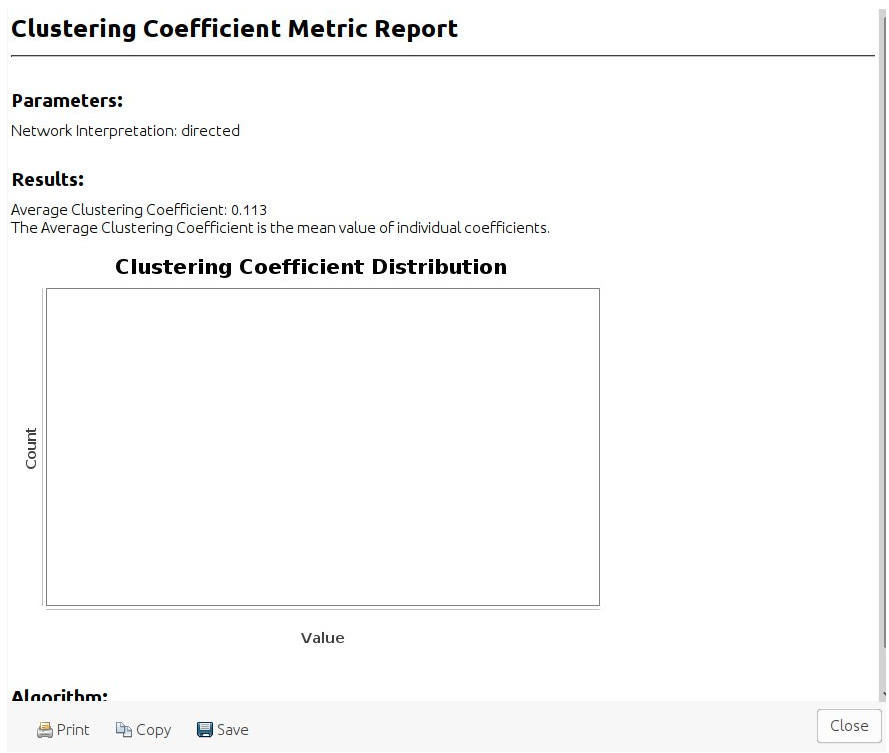
\includegraphics[width=0.5\linewidth]{Imagenes/screenshot009}
\end{figure}



\section{Cálculo de los valores de las medidas de análisis de redes sociales}
\subsection{Grado}
\begin{figure}[H]
	\centering
	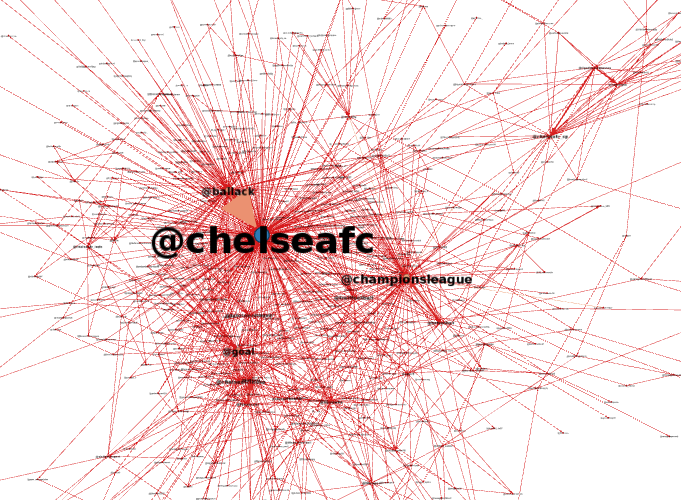
\includegraphics[width=0.6\linewidth]{Imagenes/screenshot010}
\end{figure}

Como podemos ver en la imagen, los nodos más importantes son:
\begin{itemize}
	\item @chelseafc
	\item @championsleague
	\item @goal
	\item @ballack
\end{itemize}
\subsection{Intermediación}
\begin{figure}[H]
	\centering
	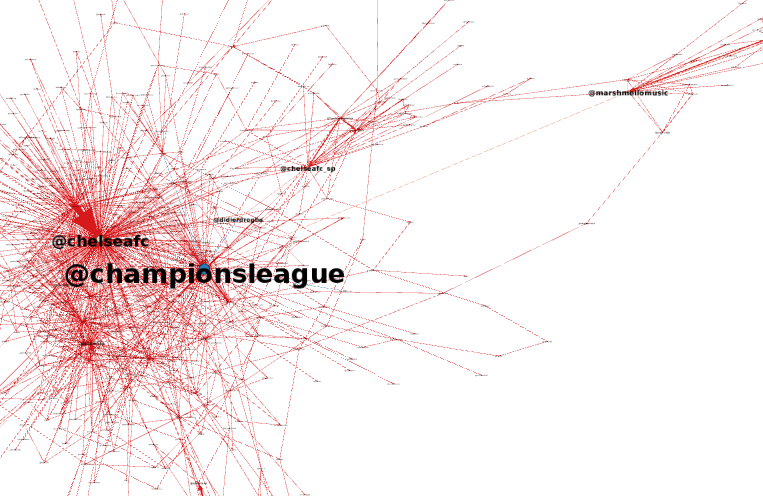
\includegraphics[width=0.7\linewidth]{Imagenes/screenshot011}
\end{figure}

En este caso, encontramos otros actores principales:
\begin{itemize}
	\item @championsleague
	\item @chelseafc
	\item @chelseafc\_sp
	\item @didierdrogba
	\item @marshmellomusic
\end{itemize}

\newpage
\subsection{Cercanía}

Como podemos ver, en este caso, son muchos los nodos que tienen el máximo tamaño (he usado una función no lineal para que se vean solo los más importantes). Por lo tanto, no tiene sentido en mi trabajo esta medida, y no ayuda a resolver las preguntas.

\begin{figure}[H]
	\centering
	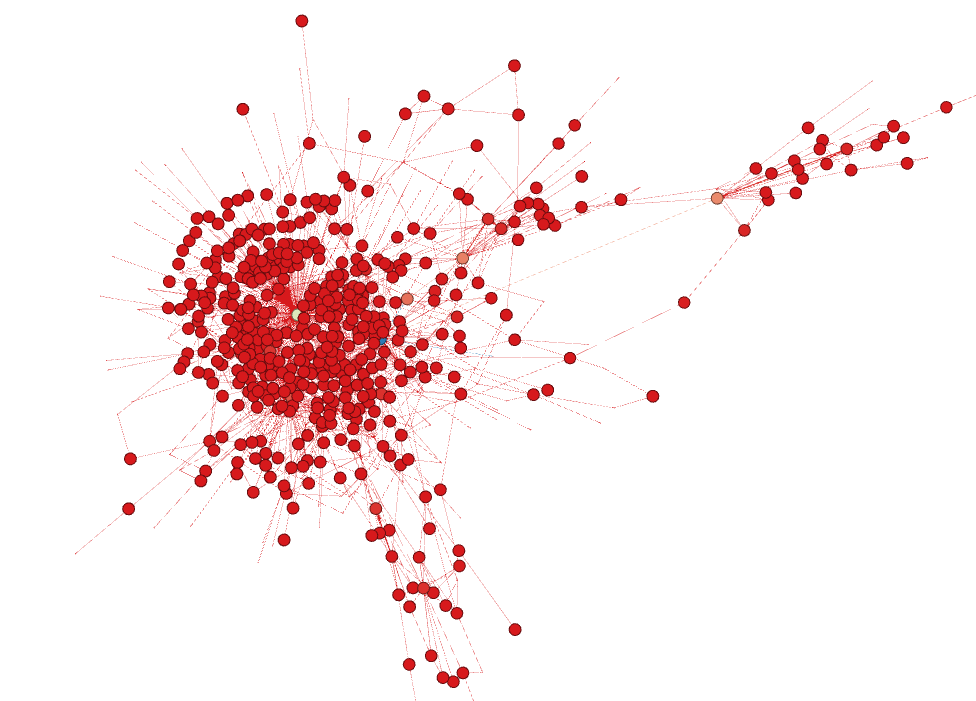
\includegraphics[width=0.7\linewidth]{Imagenes/screenshot012}
\end{figure}


\subsection{Vector propio}
Aquí vemos los nodos más valorados según el vector propio:
\begin{figure}[H]
	\centering
	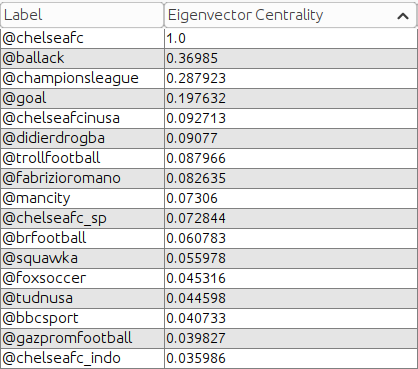
\includegraphics[width=0.6\linewidth]{Imagenes/screenshot013}
\end{figure}


\subsection{Conclusiones en cuanto a las medidas de análisis de las redes}

Según hemos visto, con las medidas anteriores, tanto el grado, la intermediación y el vector propio nos dan nodos relevantes para las preguntas que nos hemos planteado, aunque al final se detallarán más los resultados.

\section{Descubrimiento de comunidades en la red}

\subsection{Lovaina}

\begin{figure}[H]
	\centering
	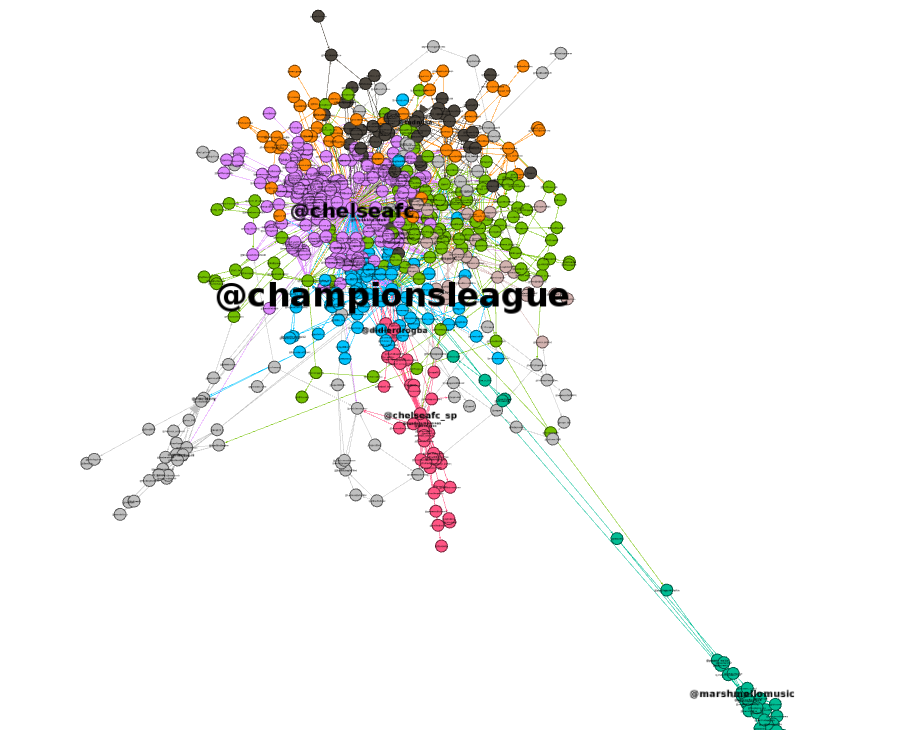
\includegraphics[width=0.7\linewidth]{Imagenes/screenshot014}
\end{figure}

Vemos que el algoritmo ha dividido en 12 las comunidades. Al ser comunidades de usuarios de tweeter, y al no conocer a estos usuarios no puedo saber exactamente si la división es correcta, pero veo alguna comunidad que está cerca de @marshmellomusic, que serán los que han estado interesados en la música del inicio de la competición, en el espectáculo que se hizo. \\
Por otro lado, vemos otro grupo de gente junto a las cuentas del Chelsea y del Chelsea en español, lo cual es muy probable que haya sucedido, que estos grupos estén diferenciados.\\
Además, vemos también gente en torno a otro nodo como puede ser @tudnusa, que es el encargado de retransmitir la Champions en EEUU, lo cual tiene sentido que exista otra comunidad en torno a él. \\
Por lo tanto, me atrevería a decir que las comunidades guardan un mínimo de sentido y nos aportan información extra a nuestro estudio.

\subsection{Girvan-Newman}
\begin{figure}[H]
	\centering
	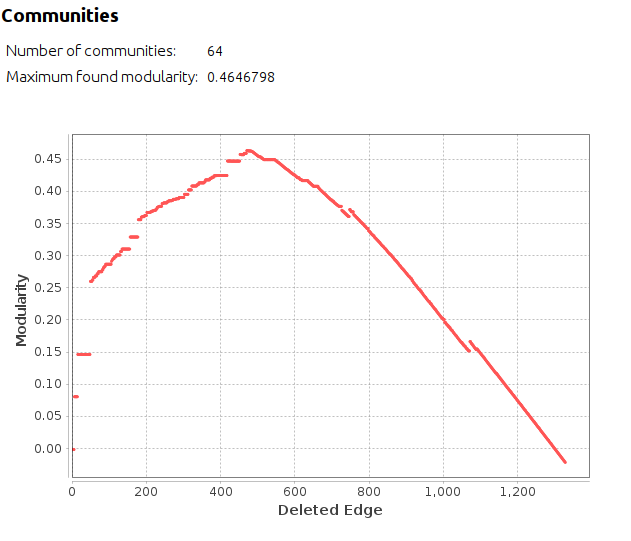
\includegraphics[width=0.7\linewidth]{Imagenes/screenshot015}
\end{figure}

Como podemos ver, el algoritmo de Girvan-Newman nos acaba de generar 64 comunidades, cinco veces más comunidades que Lovaina. Veamos si estas comunidades tienen sentido.

\begin{figure}[H]
	\centering
	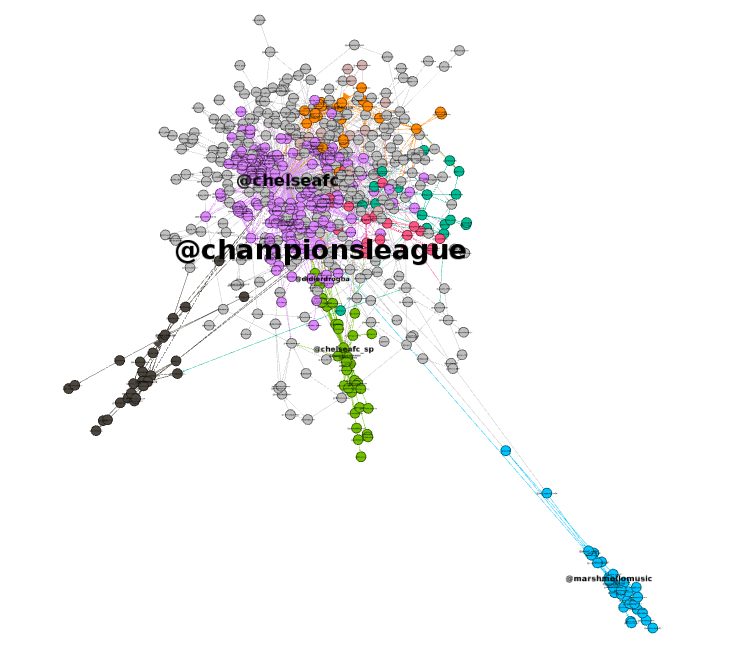
\includegraphics[width=0.7\linewidth]{Imagenes/screenshot016}
\end{figure}
Aunque a priori hemos visto que había muchas más comunidades, pero al inspeccionar más afondo descubrimos que, no solo las comunidades son muy parecidas, sino que el número tan alto de comunidades se debe a que, las comunidades de menor importancia de Lovaina han sido divididas en comunidades más pequeñas, a veces incluso comunidades de dos o tres nodos. Diría pues que Girvan-Newman nos ha dado otra visión de las comunidades, reforzando la idea de que las comunidades englobaban una identidad común y resaltando aún más las comunidades principales, quitando importancia a las comunidades menos importantes.
\newpage
\section{Visualización de la red social}
\subsection{Representación 1}


\begin{figure}[H]
	\centering
	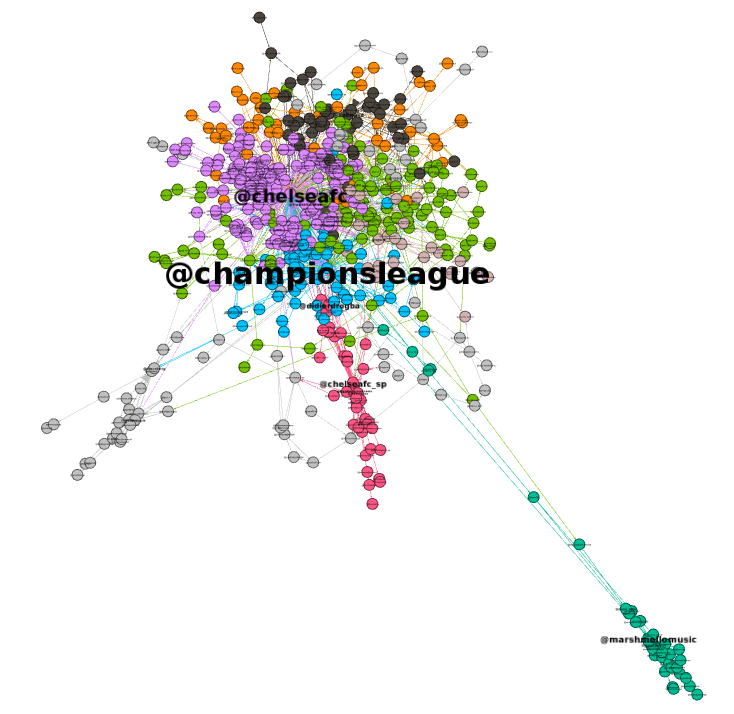
\includegraphics[width=0.75\linewidth]{Imagenes/screenshot023}
\end{figure}

En primer lugar, he usado una representación basada en Force Atlas. Como podemos observar, los nodos están coloreados por comunidades, las que hemos obtenido de Girvan-Newman, ya que me parecen relevantes. Además, para poder ver bien los nodos principales de cada comunidad, se han pintado las etiquetas con un tamaño más grande a las que tienen un mayor valor de intermediación. Como algún nodo tenía un valor devastador, como era el caso del nodo @championsleague, se ha usado una función no lineal para que este nodo non sea demasiado grande y no nos deje apreciar toda la red. La función es la siguiente:

\begin{figure}[H]
	\centering
	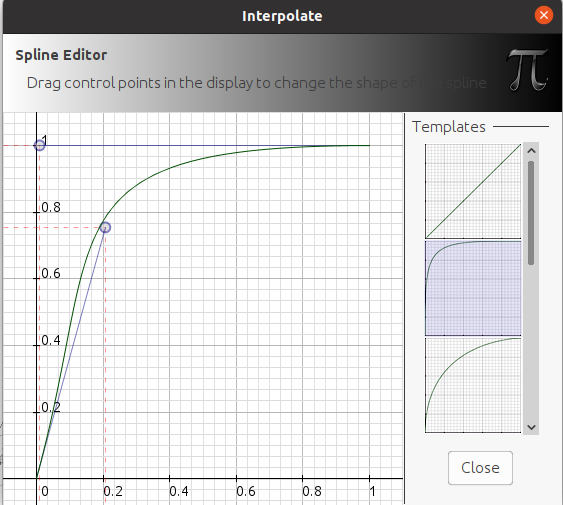
\includegraphics[width=0.25\linewidth]{Imagenes/screenshot018}
\end{figure}


\subsection{Representación 2}
\begin{figure}[H]
	\centering
	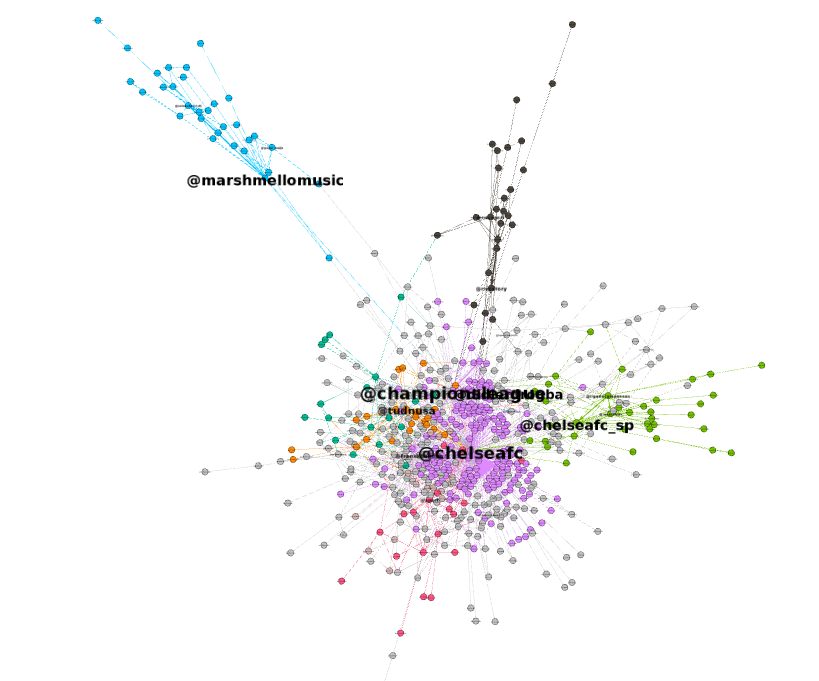
\includegraphics[width=0.7\linewidth]{Imagenes/screenshot019}
\end{figure}

Otro visualizado que he usado a lo largo de toda la práctica ha sido el proporcionado con Yifan Hu. También me parece que queda bonito y es similar al caso anterior. En este se puede apreciar un poco más que Chelsea y ChampionsLeague están más unidos y relacionados que Marshmello.
\newpage
\subsection{Easter Egg}
Por último, he querido remarcar un dato curioso, y es que, como podemos ver, hay una arista con mucho más peso que las demás. Esto es provocado por un alto número de me gustas, retwittes y comentarios. Esto es debido a que una publicación se hizo muy viral. Un ex jugador del Chelsea decidió ir a un club de alterne en lugar de ver la final de su ex-equipo, loo que hizo que la gente se mofara de ello en Twitter y saliera en nuestro particular estudio.
\begin{figure}[H]
	\centering
	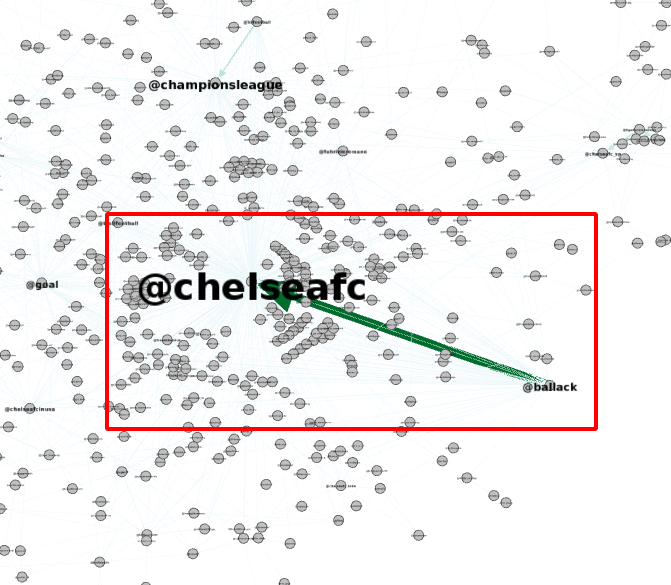
\includegraphics[width=0.7\linewidth]{Imagenes/screenshot022}
\end{figure}

\newpage
\section{Discusión de los resultados obtenidos}
En primer lugar, he de decir que he quedado bastante sorprendido de que el Manchester City no saliera como ningún nodo principal en ningún momento, aunque sí estaba entre todos los nodos que hemos estudiado. En cambio, el Chelsea hemos podido ver que ha sido un nodo muy importante y un eje central de la red en todo momento. Obviamente esto se debe a que, en el momento en que se recolectaron los datos, el Chelsea era el que acababa de marcar, y es mucho más común decir que tu equipo a marcado en vez de expresar que tu equipo ha recibido un gol.\\

La segunda sorpresa ha sido no encontrar por ningún lado el Twitter del goleador. Esto puede ser debido, nuevamente, a que los datos fueron tomados en un intervalo de tiempo muy pequeño. A día de hoy, si tuviera que repetir el experimento, habría dejado en marca la búsqueda de tweets todo el partido, aunque claro, si obtuve más de 12000 en menos de un minuto, no sé hasta que punto podría haber obtenido los tweets de todo el partido o habría registrado algún fallo, ya sea de mi ordenador o de la API (diría que hay un máximo de 50000 tweets que puedes recoger en un periodo de tiempo de un mes).\\

Por lo tanto, de las tres preguntas que inicialmente hacía, las dos últimas no se han conseguido, no ha aparecido el goleador del partido y no se ha podido distinguir la comunidad del Chelsea frente a la del Manchester City.\\

No obstante, con el estudio de esta red sencilla he sacado mucha más información de la que esperaba: gente a la que le interesó mucho más el espectáculo inicial que el partido en si mismo, gente que viralizó un tweet de una ex-estrella del Chelsea y comunidades formadas por la zona geográfica en la que se reside, unos en EEUU, otros apoyando al Chelsea desde España y por último, el grupo más multitudinario, los fans ingleses del equipo de Londres.
	
	
\end{document}